\documentclass[11pt]{article}

\usepackage{latexsym}
\usepackage{amsmath}
\usepackage{amssymb}
\usepackage{amsthm}
\usepackage{graphicx}
\usepackage{wrapfig}
\usepackage{pseudocode}
\usepackage{url}
\usepackage{float}
\usepackage{subcaption}
\usepackage{listings}
\usepackage{color}
\usepackage[backref, colorlinks=true, citecolor=red, urlcolor=blue, pdfauthor={Jyh-Ming Lien}]{hyperref}


\newcommand{\handout}[5]{
  \noindent
  \begin{center}
  \framebox{
    \vbox{
      \hbox to 5.78in { {\bf } \hfill #2 }
      \vspace{4mm}
      \hbox to 5.78in { {\Large \hfill #5  \hfill} }
      \vspace{2mm}
      \hbox to 5.78in { {\em #3 \hfill #4} }
    }
  }
  \end{center}
  \vspace*{4mm}
}

\newcommand{\lecture}[4]{\handout{#1}{#2}{#3}{#4}{#1}}

\newtheorem{theorem}{Theorem}
\newtheorem{corollary}[theorem]{Corollary}
\newtheorem{lemma}[theorem]{Lemma}
\newtheorem{observation}[theorem]{Observation}
\newtheorem{proposition}[theorem]{Proposition}
\newtheorem{definition}[theorem]{Definition}
\newtheorem{claim}[theorem]{Claim}
\newtheorem{fact}[theorem]{Fact}
\newtheorem{assumption}[theorem]{Assumption}

% 1-inch margins, from fullpage.sty by H.Partl, Version 2, Dec. 15, 1988.
\topmargin 0pt
\advance \topmargin by -\headheight
\advance \topmargin by -\headsep
\textheight 8.9in
\oddsidemargin 0pt
\evensidemargin \oddsidemargin
\marginparwidth 0.5in
\textwidth 6.5in

\parindent 0in
\parskip 1.5ex
%\renewcommand{\baselinestretch}{1.25}

\definecolor{dkgreen}{rgb}{0,0.6,0}
\definecolor{gray}{rgb}{0.5,0.5,0.5}
\definecolor{mauve}{rgb}{0.58,0,0.82}

\lstset{
	frame=tb,
	language=C++,
	aboveskip=3mm,
	belowskip=3mm,
	showstringspaces=false,
	columns=flexible,
	basicstyle={\small\ttfamily},
	numbers=none,
	numberstyle=\tiny\color{gray},
	keywordstyle=\color{blue},
	commentstyle=\color{dkgreen},
	stringstyle=\color{mauve},
	breaklines=true,
	breakatwhitespace=true,
	tabsize=3
}
														
\begin{document}

\lecture{Voronoi Stippling Report}{Fall 2017}{Stephen Arnold - G00864316}{CS633 - Computational Geometry}

\section{Summary of the Two Methods}
In this introductory section, the methods and algorithms employed by the two stippling techniques shall be reviewed.

\subsection{Voronoi Method}
The provided implementation of Voronoi (VR) stippling makes use of Fortune's Algorithm for the calculation of the Voronoi Cells. Initially, the input parameters are read in and stored. Next, an initial random distribution of points is created within the boundaries of the original image. These data points are the initial configuration stored in the stippler data structure.

Using an iterative approach, a Voronoi Diagram is created from the set of inital points using Fortune's Algorithm. Next, the applied stipples are redistributed and the displacement from the new locations to the previous centroids is calculated. This process is repeated until the average change in displacements across all cell meets a minimum threshold. Once the centroids have settled, the image is stippled by placing circles sized in proportion to the number of iterations required to refine the Voronoi Cell centroid.

\subsection{Hedcuter Method}
Using an iterative approach, the hedcuter (HC) stippler uses simple rejection sampling to generate an initial distribution of points, or centroids, within the confines of a given image. The algorithm compares the grayscale value of the randomly selected location within the image and applies a gaussian scaling factor. The point is either accepted or rejected based on satisfying a predetermined threshold - namely the grayscale value of the pixel. Once the inital points are determined, a set of right cones are generated with apexes at the cell generator. Initially the cones have equal height. Each cone is also assigned a unique "color" to identify it later. The intersection of the cones in the z-direction will determine to which cone the pixels of the original image belong. In this way, the pixels are assigned a unique value which determines to which Voronoi Cell the pixels belong.

The weighted Centroidal Voronoi Tessellation (CVT) used by the hedcuter algorithm makes use of a density function to distribute, and realign, the centroids of the Voronoi Diagram. Darker areas (lines, edges, etc.) are assigned a higher density than lighter areas. As the algorithm iterates through the image, centroids tend to migrate towards higher density regions.

The stippling method invoked by the hedcuter places a variably sized disk, centered at the centroid of the cell. Two options exist within the code: uniformly sized disks and variably-sized disks. Various levels of gray may be obtained by uniform-sized disks at varoius spacing densities or by varying the sizes of the placed disks. Colored disks may also be used in conjunction to create various tones. \cite{Secord:2002:WVS:508530.508537}

\section{Comparison of the two methods}
After compilation of both stippling methods, various test cases were run to compare each methods effectiveness as a stippling method. Those results shall be discussed here.

A single image was used to allow for simple comparrison of the significant variables of interest. The image, seen in Figure \ref{fig:AbrahamLincoln}, is a grayscale PNG-format  image of Abraham Lincoln, 16th president of the United States, from the year 1865. The image size is 1332px x 1644px, and is composed of 256 levels of grayscale. Unless otherwise noted, this image was used for all variations.

\begin{figure}[H]
	\centering
	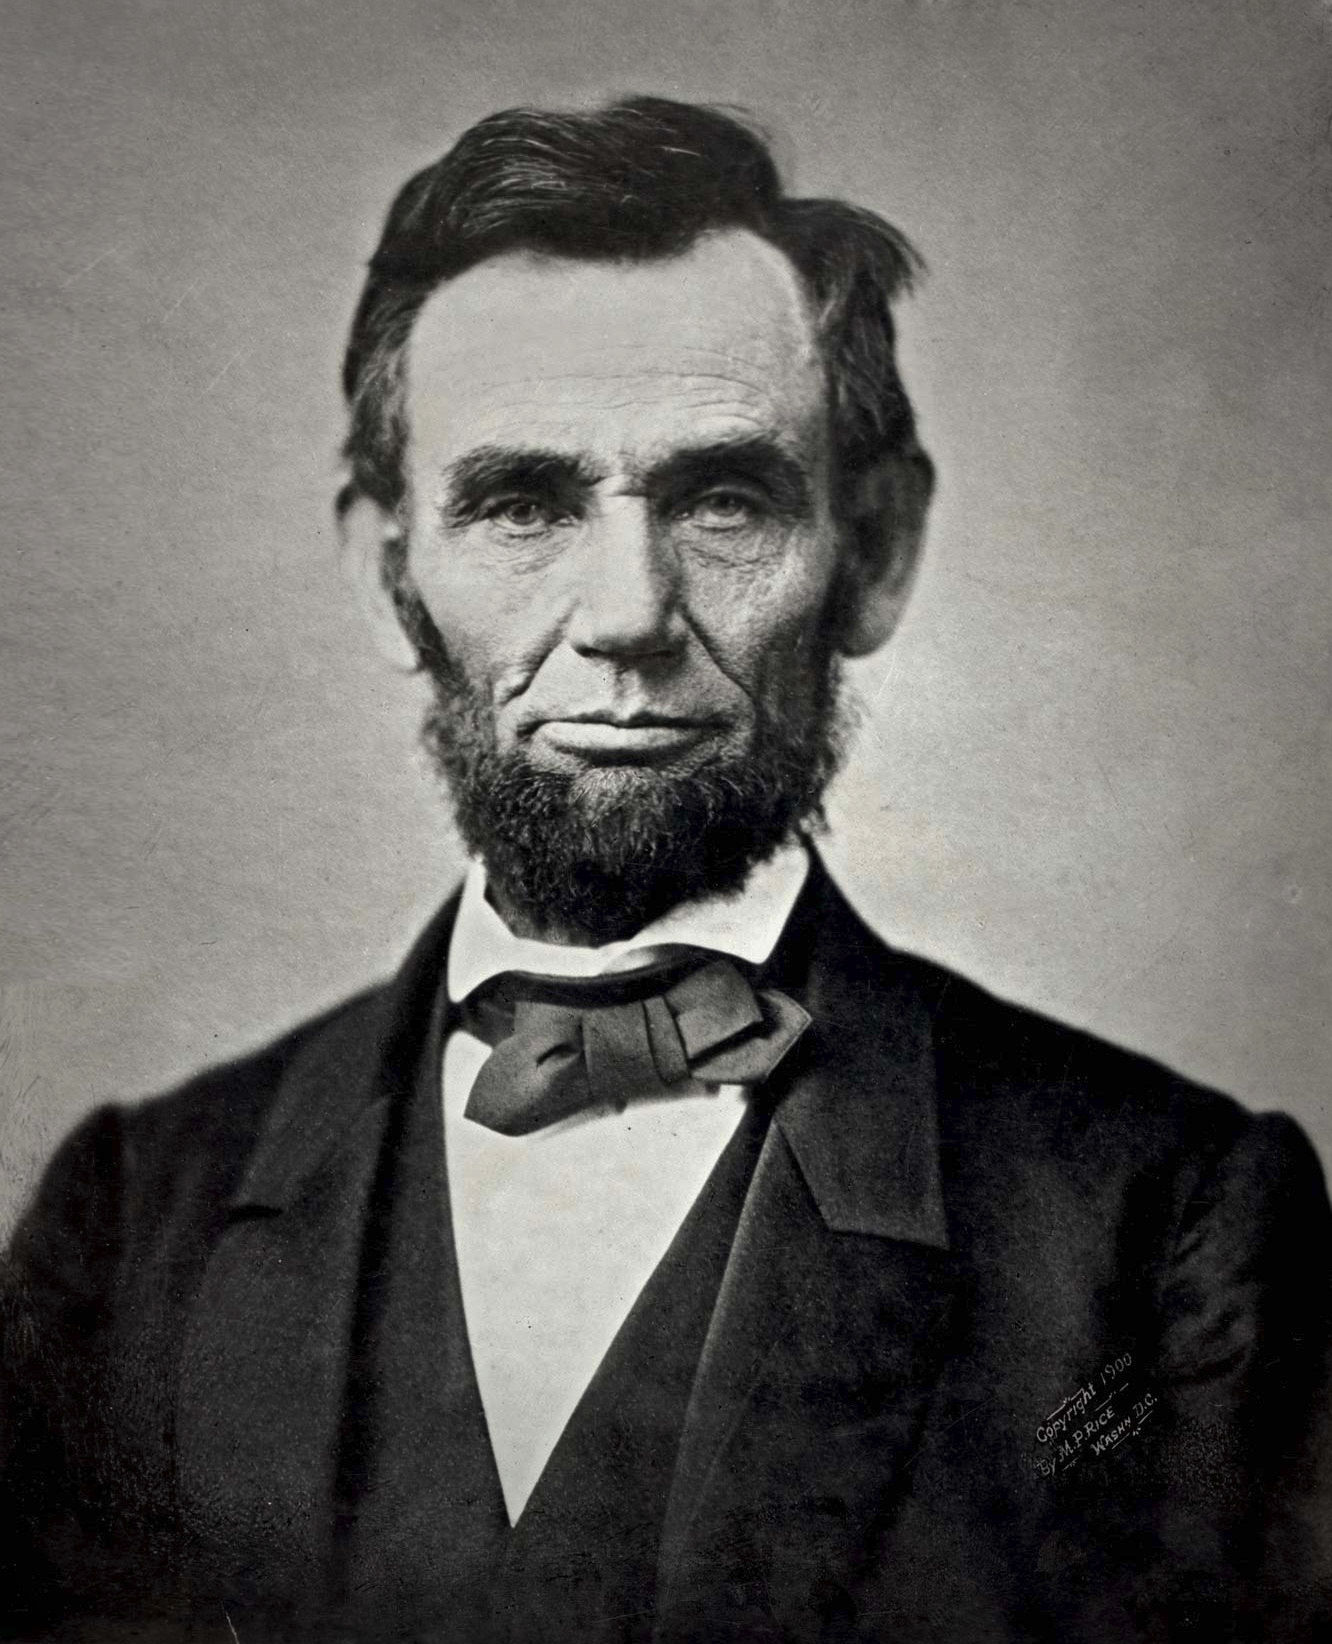
\includegraphics[width=0.5\linewidth]{pix/Abraham_Lincoln_November_1863.png}
	\caption{Abraham Lincoln, 1865.}
	\label{fig:AbrahamLincoln}
\end{figure}

\subsection{Multipass Results}
To determine if there are any statistically significant variations in running the same program on the same image multiple times, a script was written to test this condition. For VM, the results of each run using 4000 points, subpixel density 5, non-overlapping, and variable radius were extremely consistent. Minor variations in the duration of the runs were seen. Over 5 runs, times ranged from 56.78 to 57.28 seconds. Of note, when visually comparing the VM processed images, no descernable differences in final pixel placement are found. This is due to the approached used to shift the centroid of the Voronoi Cell - initially determined from random selection of points within the image. The shifting is based on actual color values of nearby pixels. Eventually the centroids will converge to similar points.

For a similar run using HC, using 4000 points, max disk size of 5, and non-uniform disk sizing, program run times ranged from 263.41 to 453.37 seconds. This variation is times is most likely due to the tight constraints of the Point select/reject function.Also, using HC results in differing placement of disks in the final image. The initial selection of points uses a probabilistic approach in determining the voronoi cell centroids. These centroids then produce selection cones in a psudo z-axis to properly assign pixels to a particular voronoi cell. The selection cones, having their apex at randomly selected locations can produce differing end result. These pixel differences can be seen in Figure \ref{fig:differences1}. These minor variations would become less pronounced at higher pixel densities.

\begin{figure}[H]
	\centering
	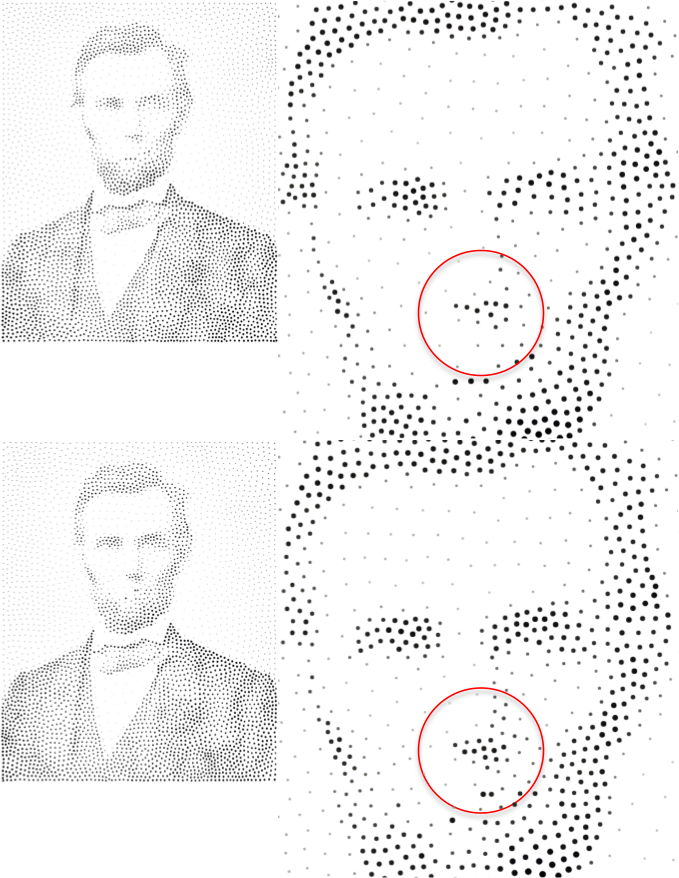
\includegraphics[width=0.5\linewidth]{pix/2-1_hc_differences.png}
	\caption{Pixel placement differences between hedcuter runs.}
	\label{fig:differences1}
\end{figure}

\subsection{Variations on Number of Disks}
Varying the number of disks has some effect on the final output images produced by the two algorithms. For voronoi, the original disk is present in its former location, but is a reduced size and has additional (also smaller) neighbors to account for the greater quantity. Also, during the initial step of the hedcuter algorithm, randomly sampled points are either selected or rejected based on a Gaussian Probability distribution against the "darkness" of a given pixel. Since both the selected point and whether or not the point will be accepted/rejected can lead to different distributions ... and can consequently explain the differences in completion times of the hedcutter algorithm.

\begin{figure}[H]
	\centering
	\begin{subfigure}[b]{0.2\linewidth}
		
\includegraphics[width=\linewidth]{pix/hc_AL_1000_r1.png}
		\caption{1000px, r=1}
	\end{subfigure}
	\begin{subfigure}[b]{0.2\linewidth}
		
\includegraphics[width=\linewidth]{pix/hc_AL_2000_r1.png}
		\caption{2000px, r=1}
	\end{subfigure}
	\begin{subfigure}[b]{0.2\linewidth}
		
\includegraphics[width=\linewidth]{pix/hc_AL_4000_r1.png}
		\caption{4000px, r=1}
	\end{subfigure}
	\begin{subfigure}[b]{0.2\linewidth}
		
\includegraphics[width=\linewidth]{pix/hc_AL_8000_r1.png}
		\caption{8000px, r=1}
	\end{subfigure}
	\begin{subfigure}[b]{0.2\linewidth}
		
\includegraphics[width=\linewidth]{pix/hc_AL_1000_r5.png}
		\caption{1000px, r=5}
	\end{subfigure}
	\begin{subfigure}[b]{0.2\linewidth}
		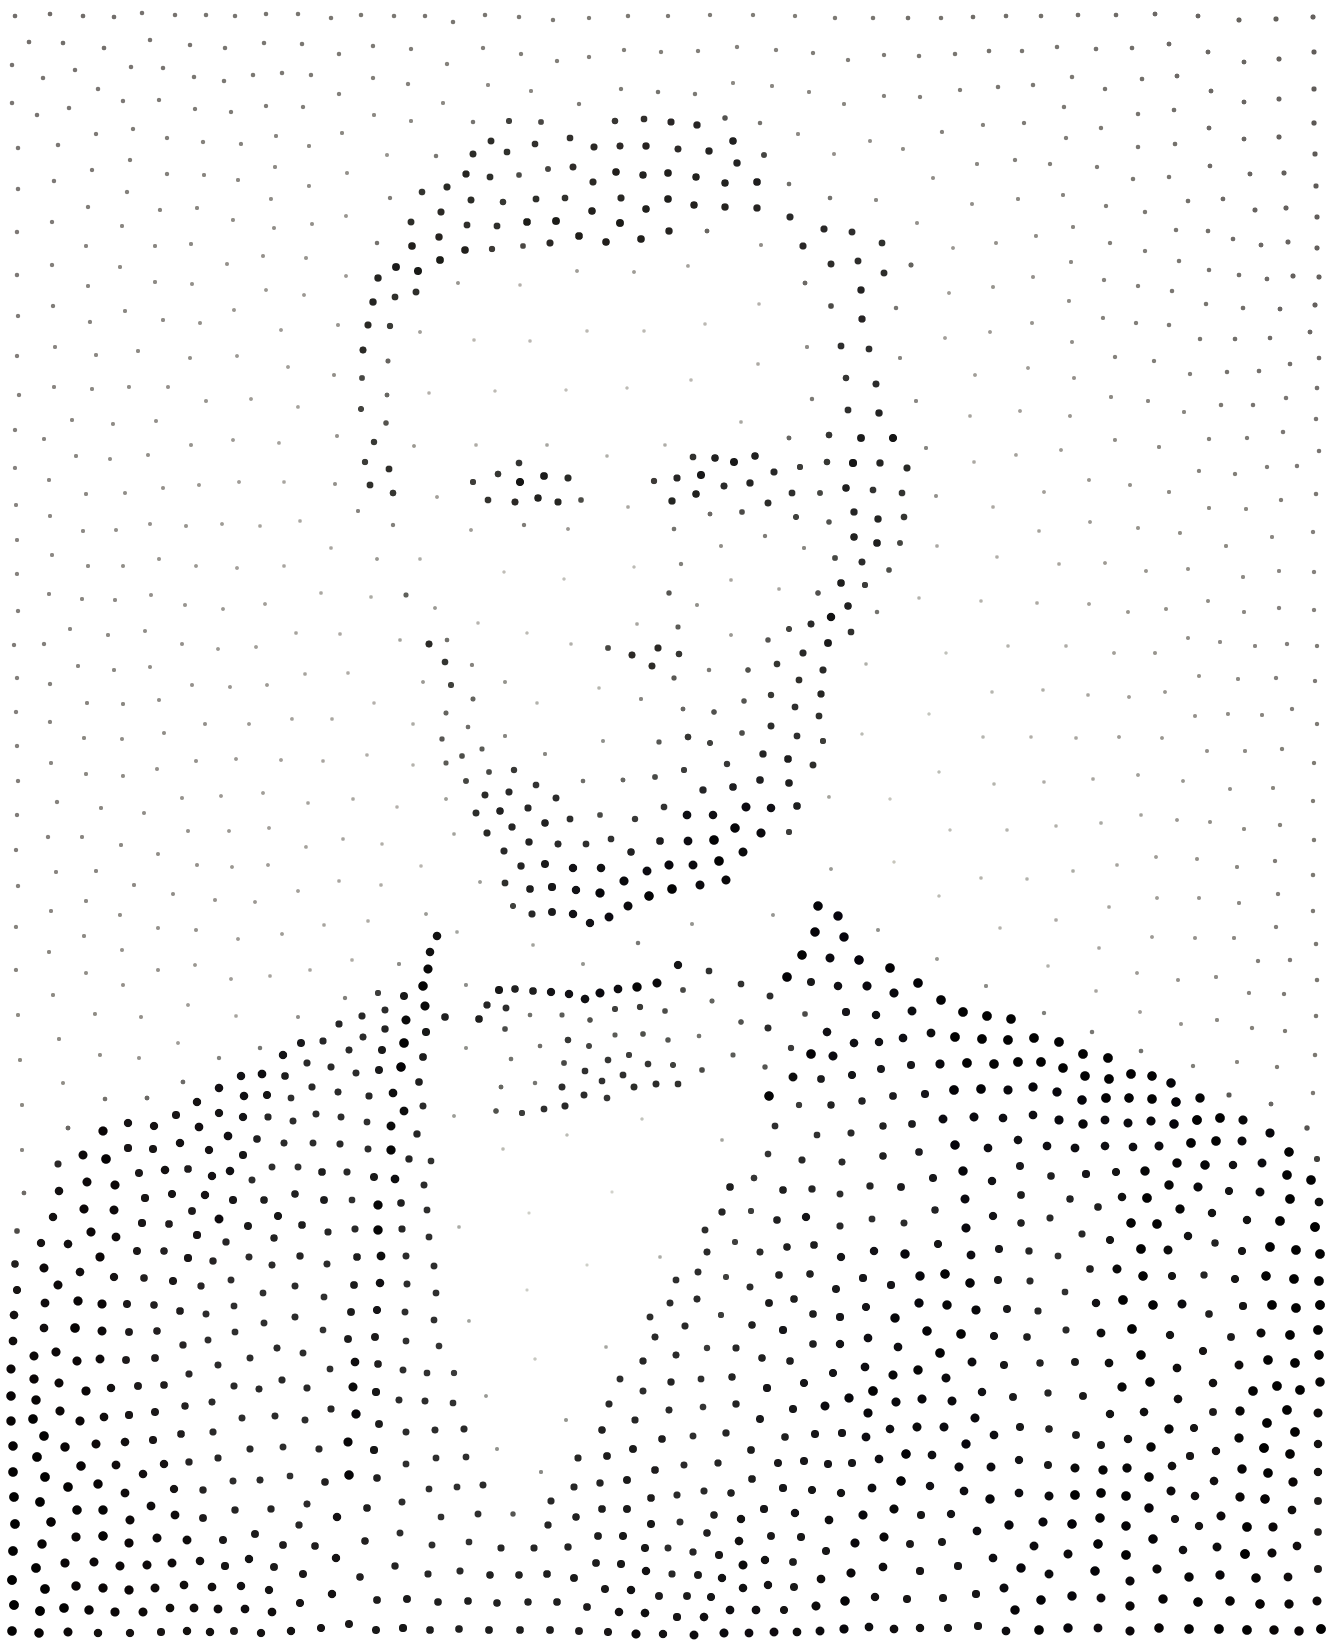
\includegraphics[width=\linewidth]{pix/hc_AL_2000_r5.png}
		\caption{2000px, r=5}
	\end{subfigure}
	\begin{subfigure}[b]{0.2\linewidth}
		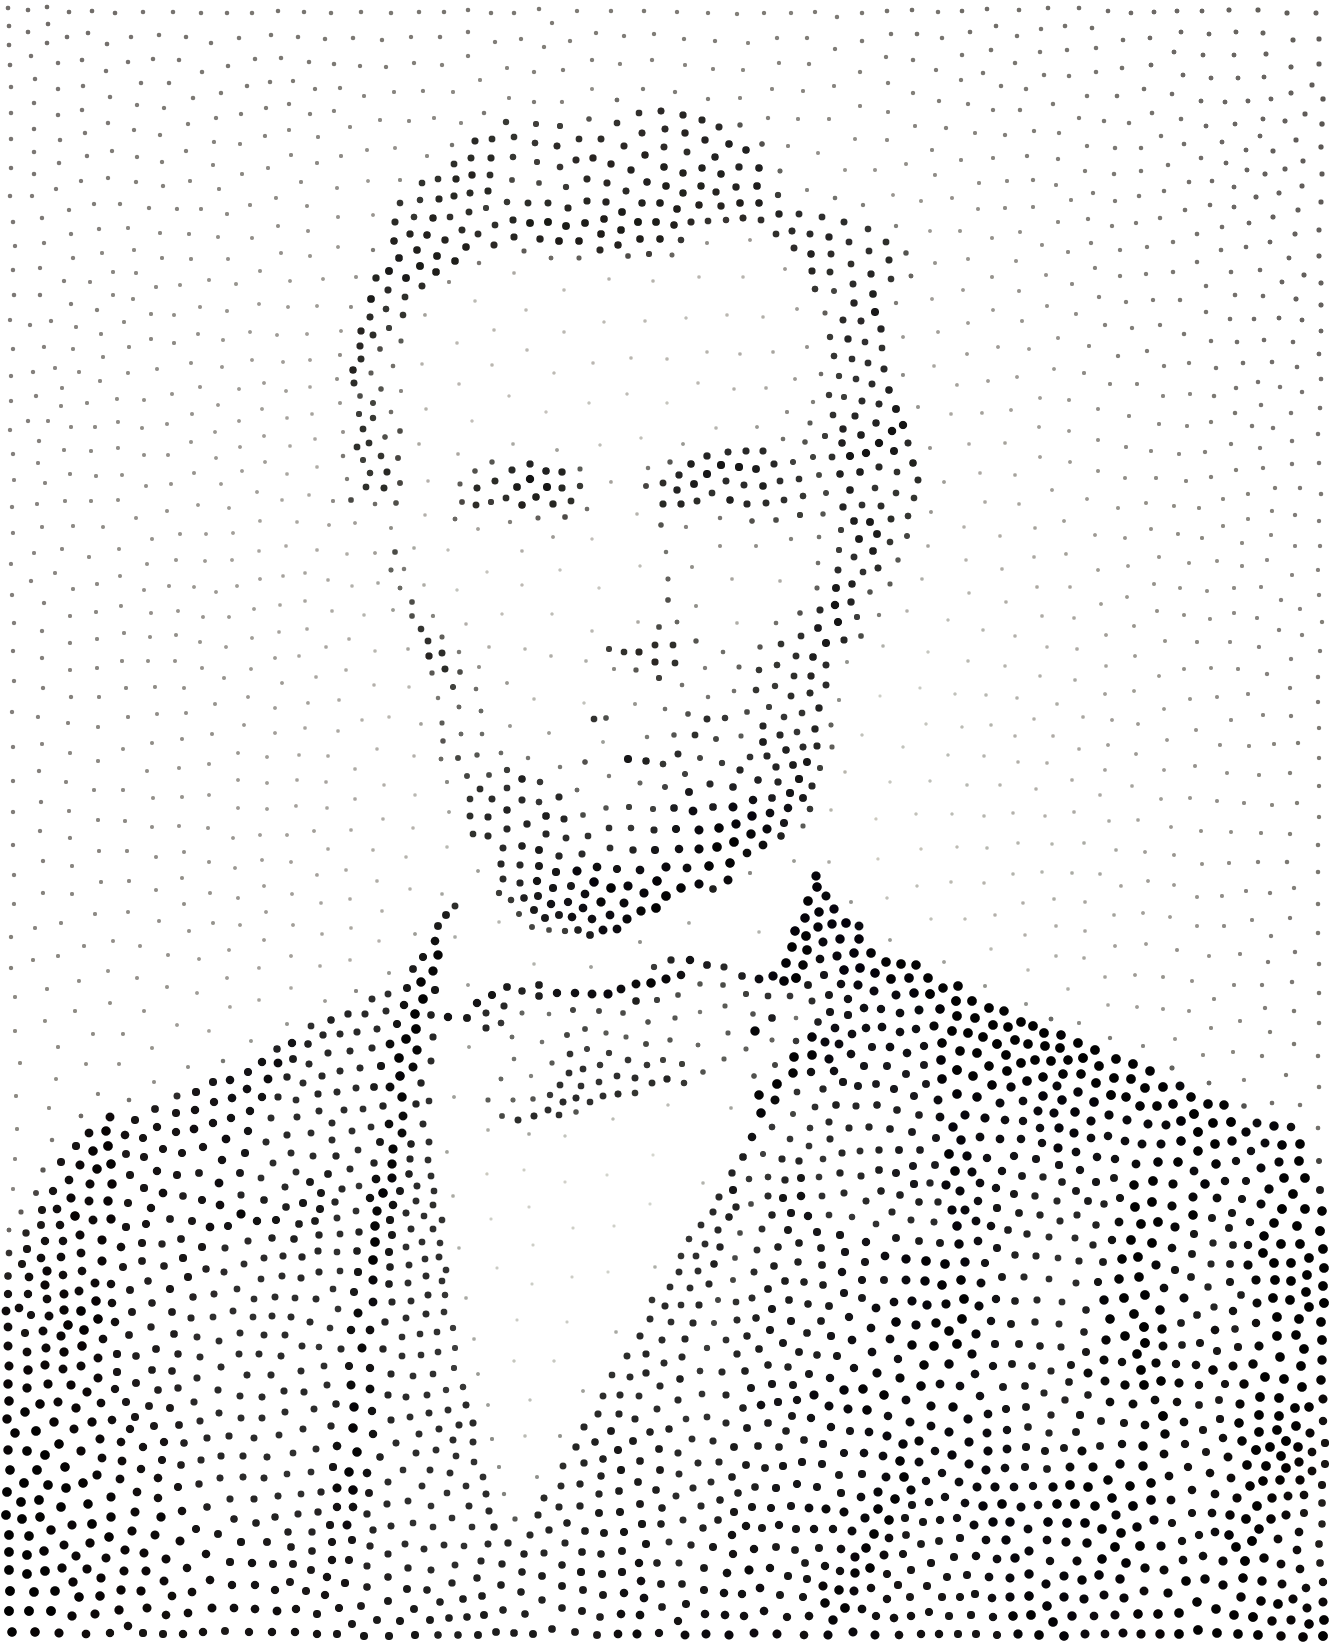
\includegraphics[width=\linewidth]{pix/hc_AL_4000_r5.png}
		\caption{4000px, r=5}
	\end{subfigure}
	\begin{subfigure}[b]{0.2\linewidth}
		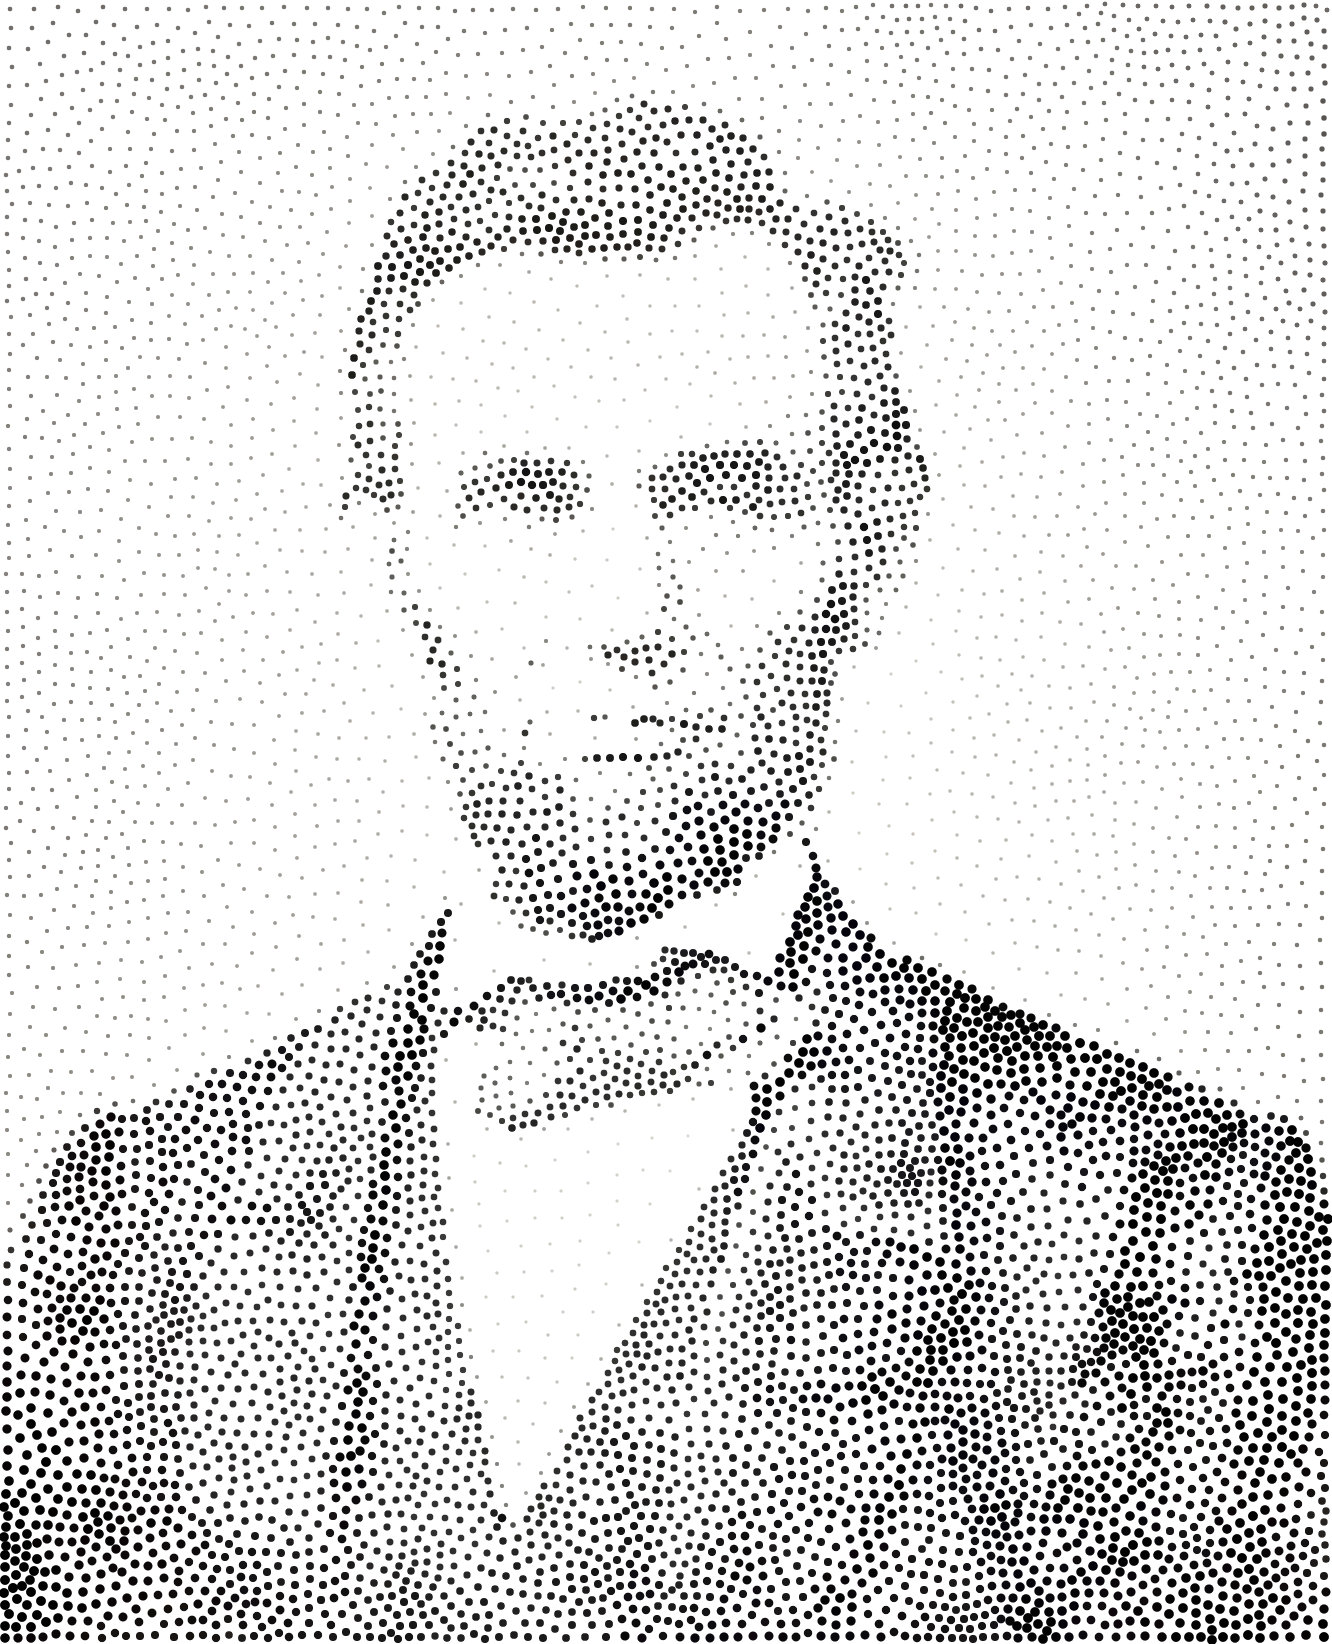
\includegraphics[width=\linewidth]{pix/hc_AL_8000_r5.png}
		\caption{8000px, r=5}
	\end{subfigure}
	\begin{subfigure}[b]{0.2\linewidth}
		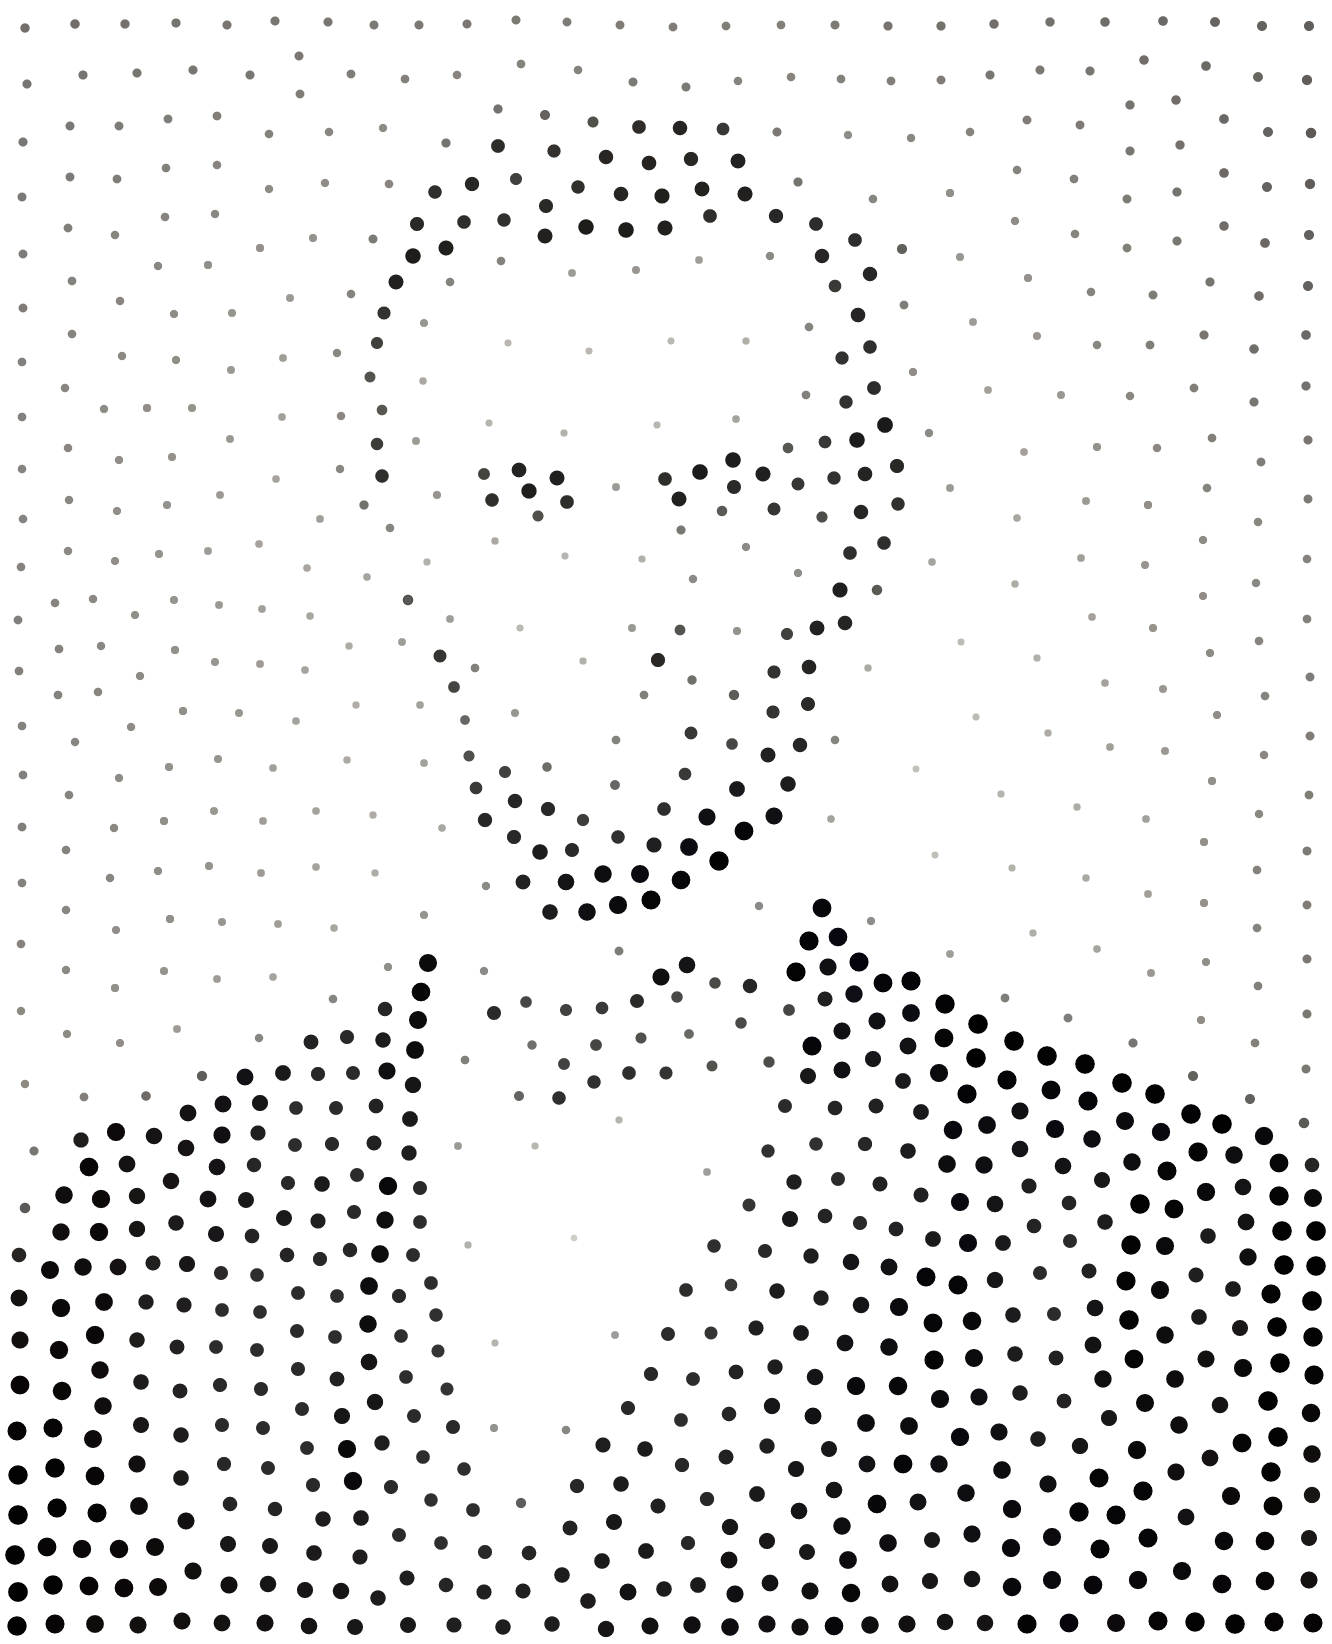
\includegraphics[width=\linewidth]{pix/hc_AL_1000_r10.png}
		\caption{1000px, r=10}
	\end{subfigure}
	\begin{subfigure}[b]{0.2\linewidth}
		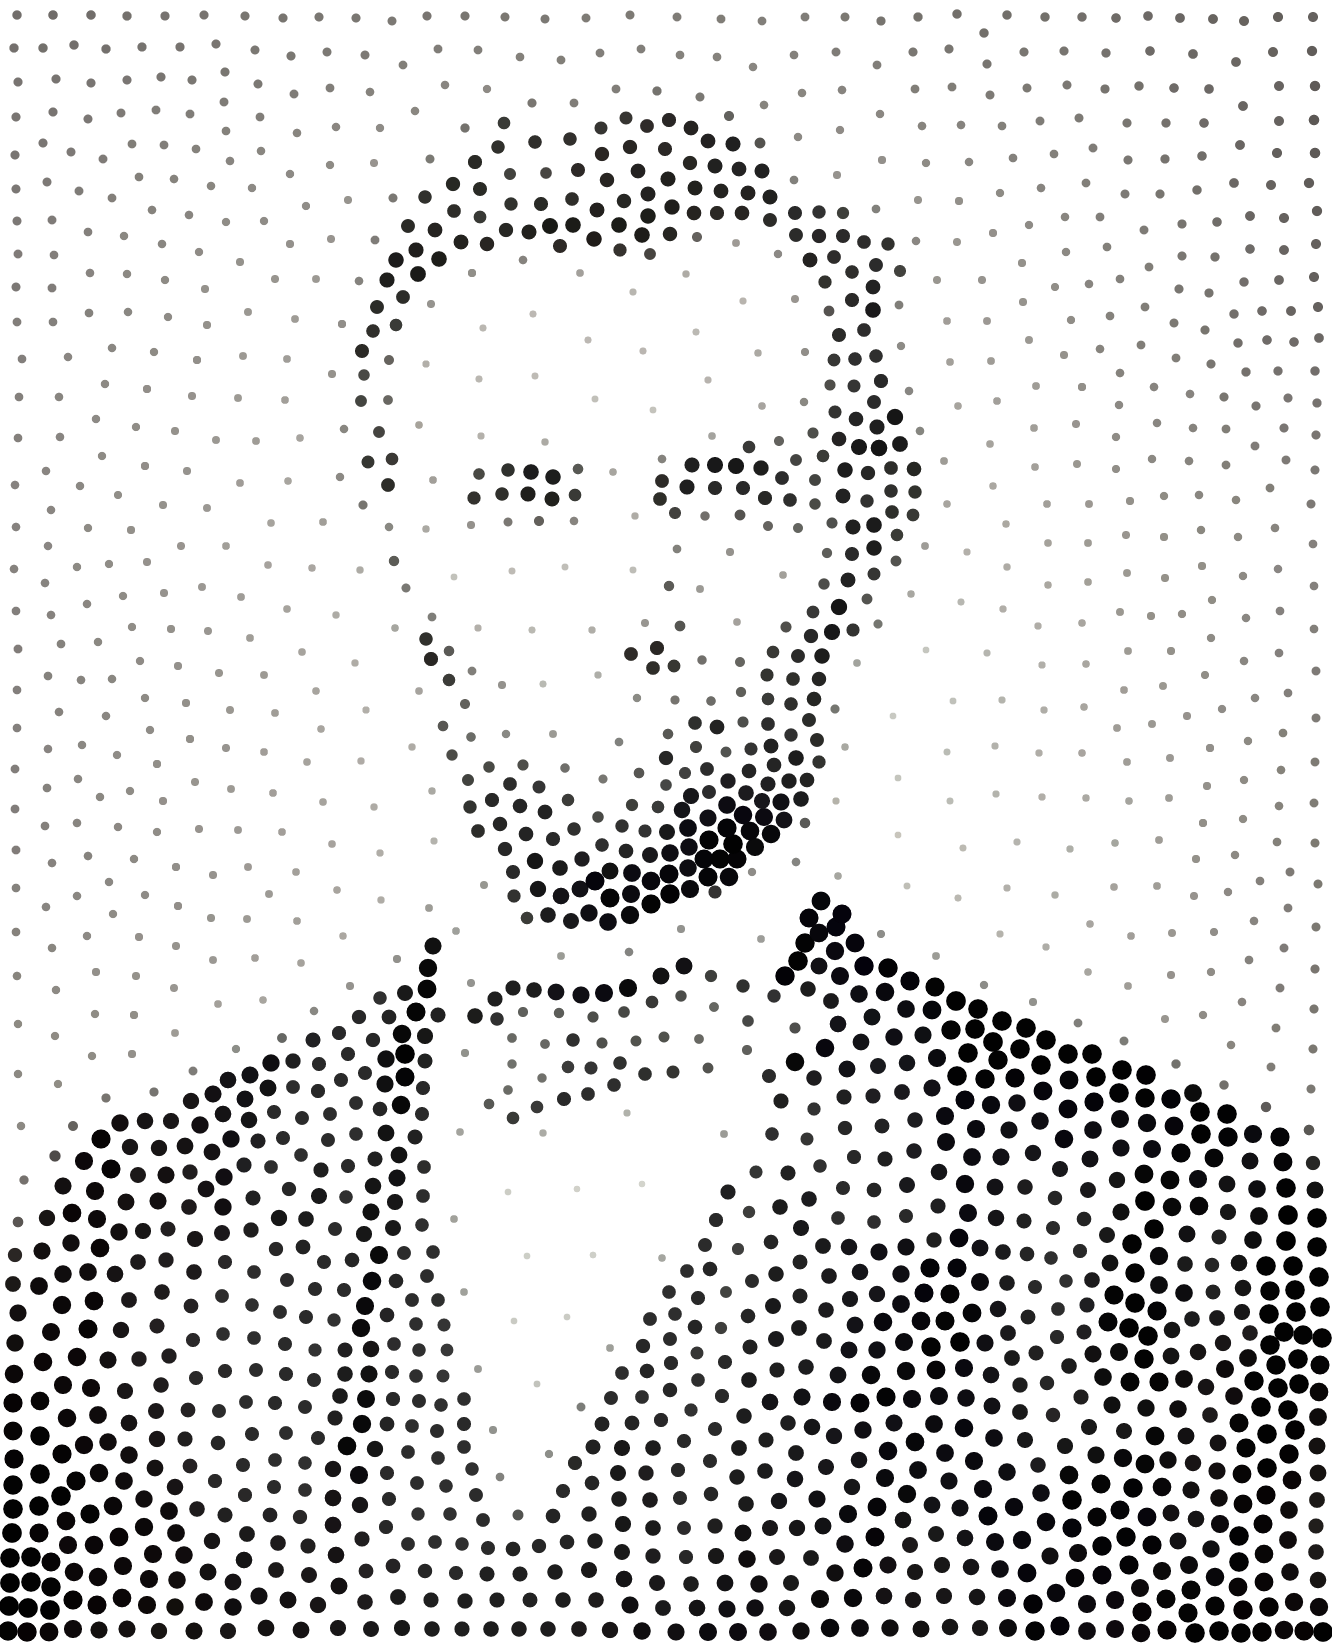
\includegraphics[width=\linewidth]{pix/hc_AL_2000_r10.png}
		\caption{2000px, r=10}
	\end{subfigure}
	\begin{subfigure}[b]{0.2\linewidth}
		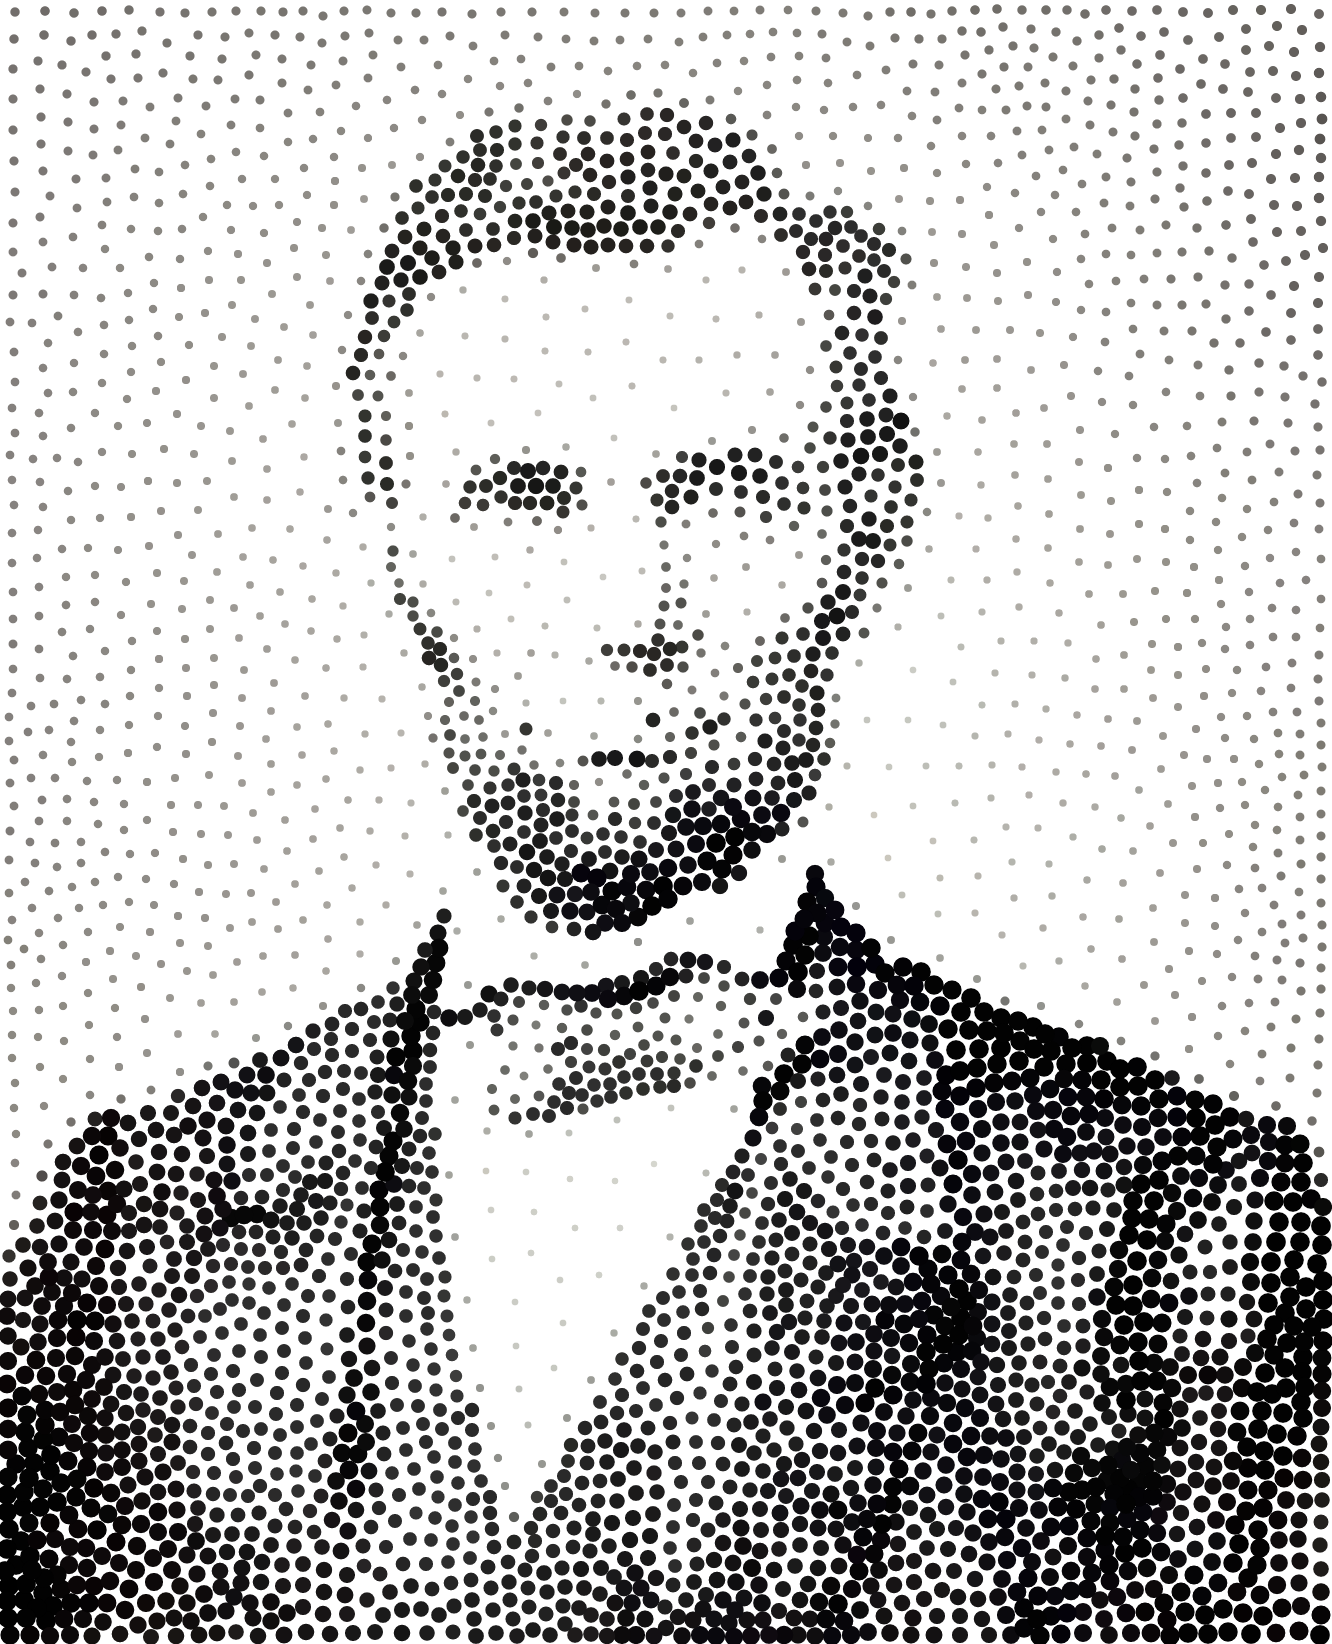
\includegraphics[width=\linewidth]{pix/hc_AL_4000_r10.png}
		\caption{4000px, r=10}
	\end{subfigure}
	\begin{subfigure}[b]{0.2\linewidth}
		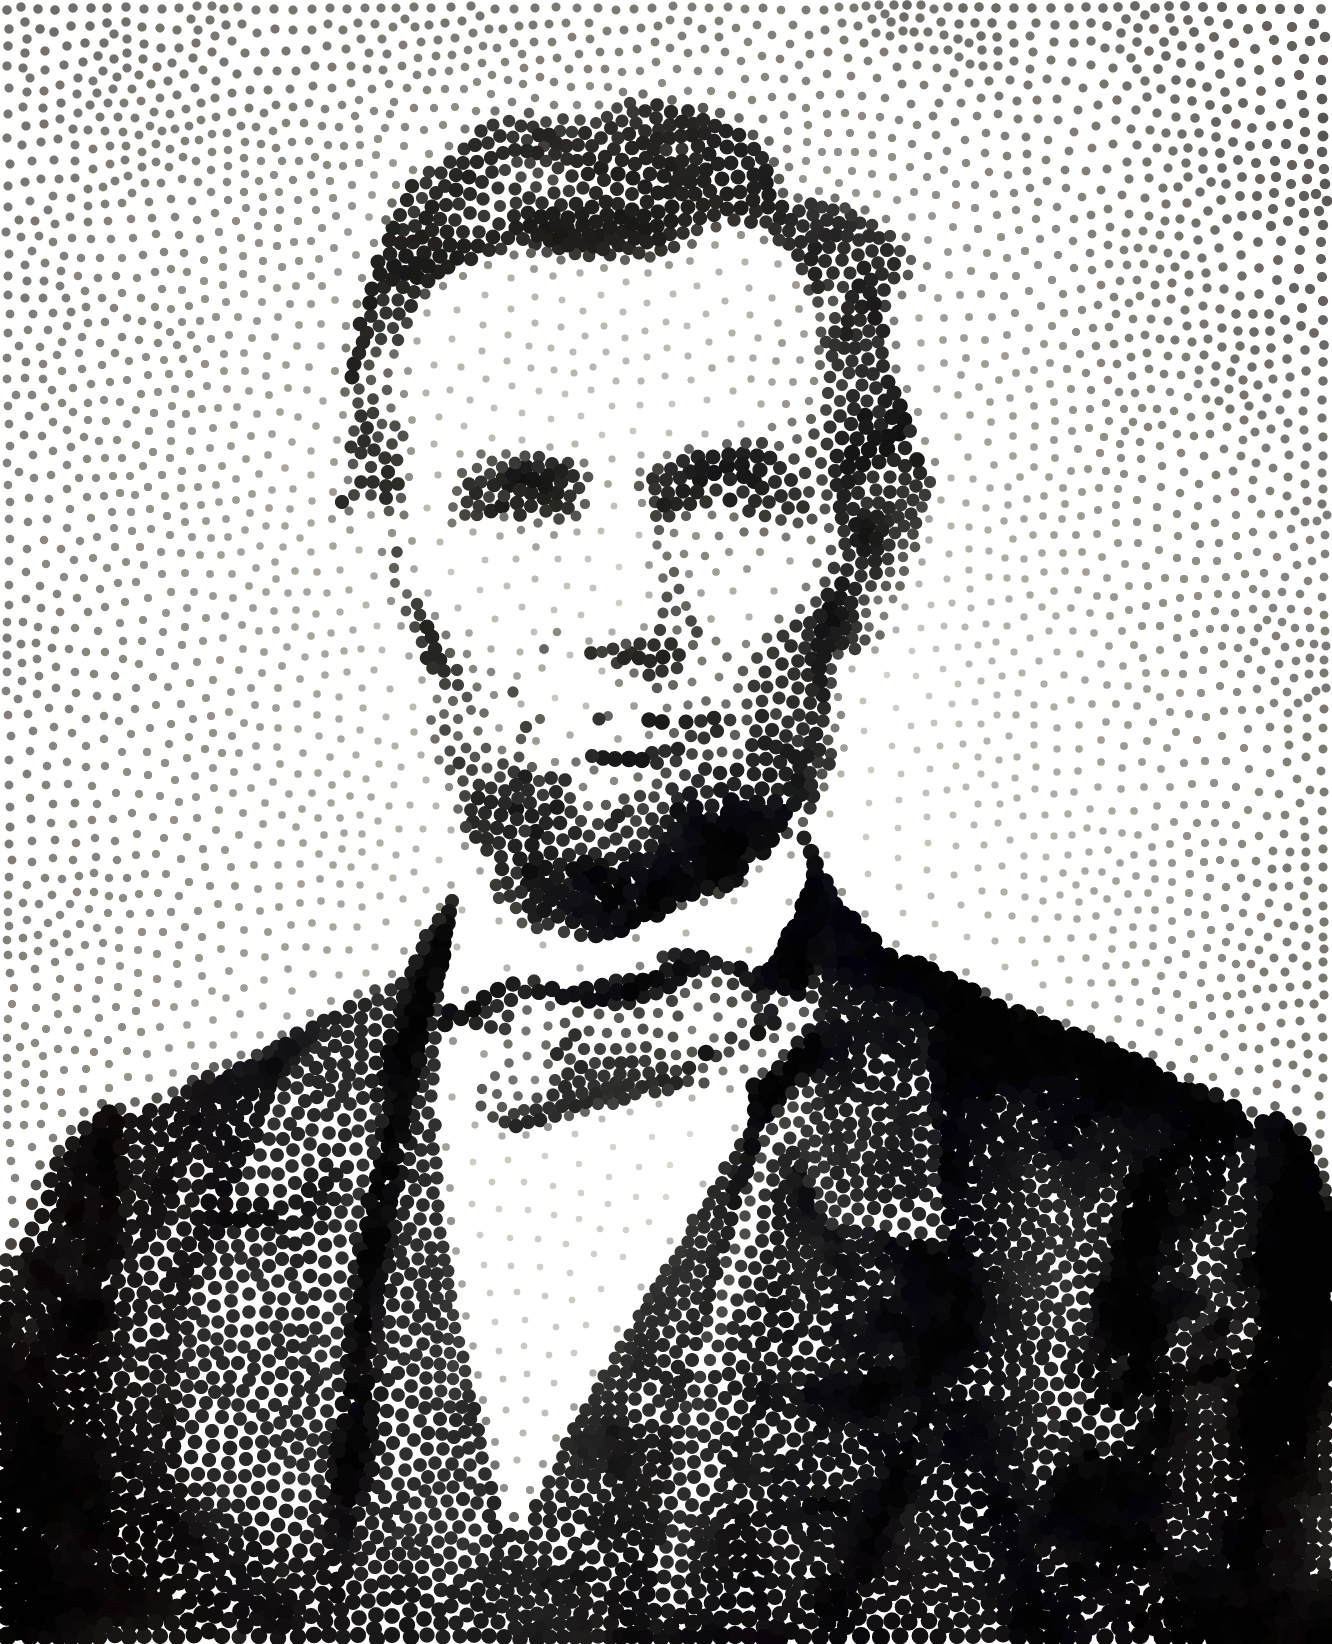
\includegraphics[width=\linewidth]{pix/hc_AL_8000_r10.png}
		\caption{8000px, r=10}
	\end{subfigure}
	\caption{Hedcuter Method images varying number of disks and radii.}
	\label{fig:hc_points1}
\end{figure}

The first row of images output from HCM in Figure \ref{fig:hc_points1} at first appears to contain no images, when in reality we have simply selected a disk size that is so small as to not be visible at the scale presented. However, in subsequent images, the stippled images may be seen progressing from least-densely to most-densely filled. 


\begin{figure}[H]
	\centering
	\begin{subfigure}[b]{0.2\linewidth}
		
\includegraphics[width=\linewidth]{pix/vr_AL_1000_r1.png}
		\caption{1000px, r=1}
	\end{subfigure}
	\begin{subfigure}[b]{0.2\linewidth}
		
\includegraphics[width=\linewidth]{pix/vr_AL_2000_r1.png}
		\caption{2000px, r=1}
	\end{subfigure}
	\begin{subfigure}[b]{0.2\linewidth}
		
\includegraphics[width=\linewidth]{pix/vr_AL_4000_r1.png}
		\caption{4000px, r=1}
	\end{subfigure}
	\begin{subfigure}[b]{0.2\linewidth}
		
\includegraphics[width=\linewidth]{pix/vr_AL_8000_r1.png}
		\caption{8000px, r=1}
	\end{subfigure}
	\begin{subfigure}[b]{0.2\linewidth}
		
\includegraphics[width=\linewidth]{pix/vr_AL_1000_r5.png}
		\caption{1000px, r=5}
	\end{subfigure}
	\begin{subfigure}[b]{0.2\linewidth}
		
\includegraphics[width=\linewidth]{pix/vr_AL_2000_r5.png}
		\caption{2000px, r=5}
	\end{subfigure}
	\begin{subfigure}[b]{0.2\linewidth}
		
\includegraphics[width=\linewidth]{pix/vr_AL_4000_r5.png}
		\caption{4000px, r=5}
	\end{subfigure}
	\begin{subfigure}[b]{0.2\linewidth}
		
\includegraphics[width=\linewidth]{pix/vr_AL_8000_r5.png}
		\caption{8000px, r=5}
	\end{subfigure}
	\begin{subfigure}[b]{0.2\linewidth}
		
\includegraphics[width=\linewidth]{pix/vr_AL_1000_r10.png}
		\caption{1000px, r=10}
	\end{subfigure}
	\begin{subfigure}[b]{0.2\linewidth}
		
\includegraphics[width=\linewidth]{pix/vr_AL_2000_r10.png}
		\caption{2000px, r=10}
	\end{subfigure}
	\begin{subfigure}[b]{0.2\linewidth}
		
\includegraphics[width=\linewidth]{pix/vr_AL_4000_r10.png}
		\caption{4000px, r=10}
	\end{subfigure}
	\begin{subfigure}[b]{0.2\linewidth}
		
\includegraphics[width=\linewidth]{pix/vr_AL_8000_r10.png}
		\caption{8000px, r=10}
	\end{subfigure}
	\caption{Voronoi Method images varying number of disks and radii.}
	\label{fig:vc_points1}
\end{figure}

The images produced by VR, and seen in Figure \ref{fig:vc_points1}, demonstrate the constrain of disk size based on localized grayscale value. Regardless of the limitation of the tile size of centroid computations, the variations are iteratively removed as the algorithm progresses. The variably sized stipple points allow finer details such as edges or textures to be preserved.

\begin{figure}[H]
	\centering
	\begin{subfigure}[b]{0.4\linewidth}
		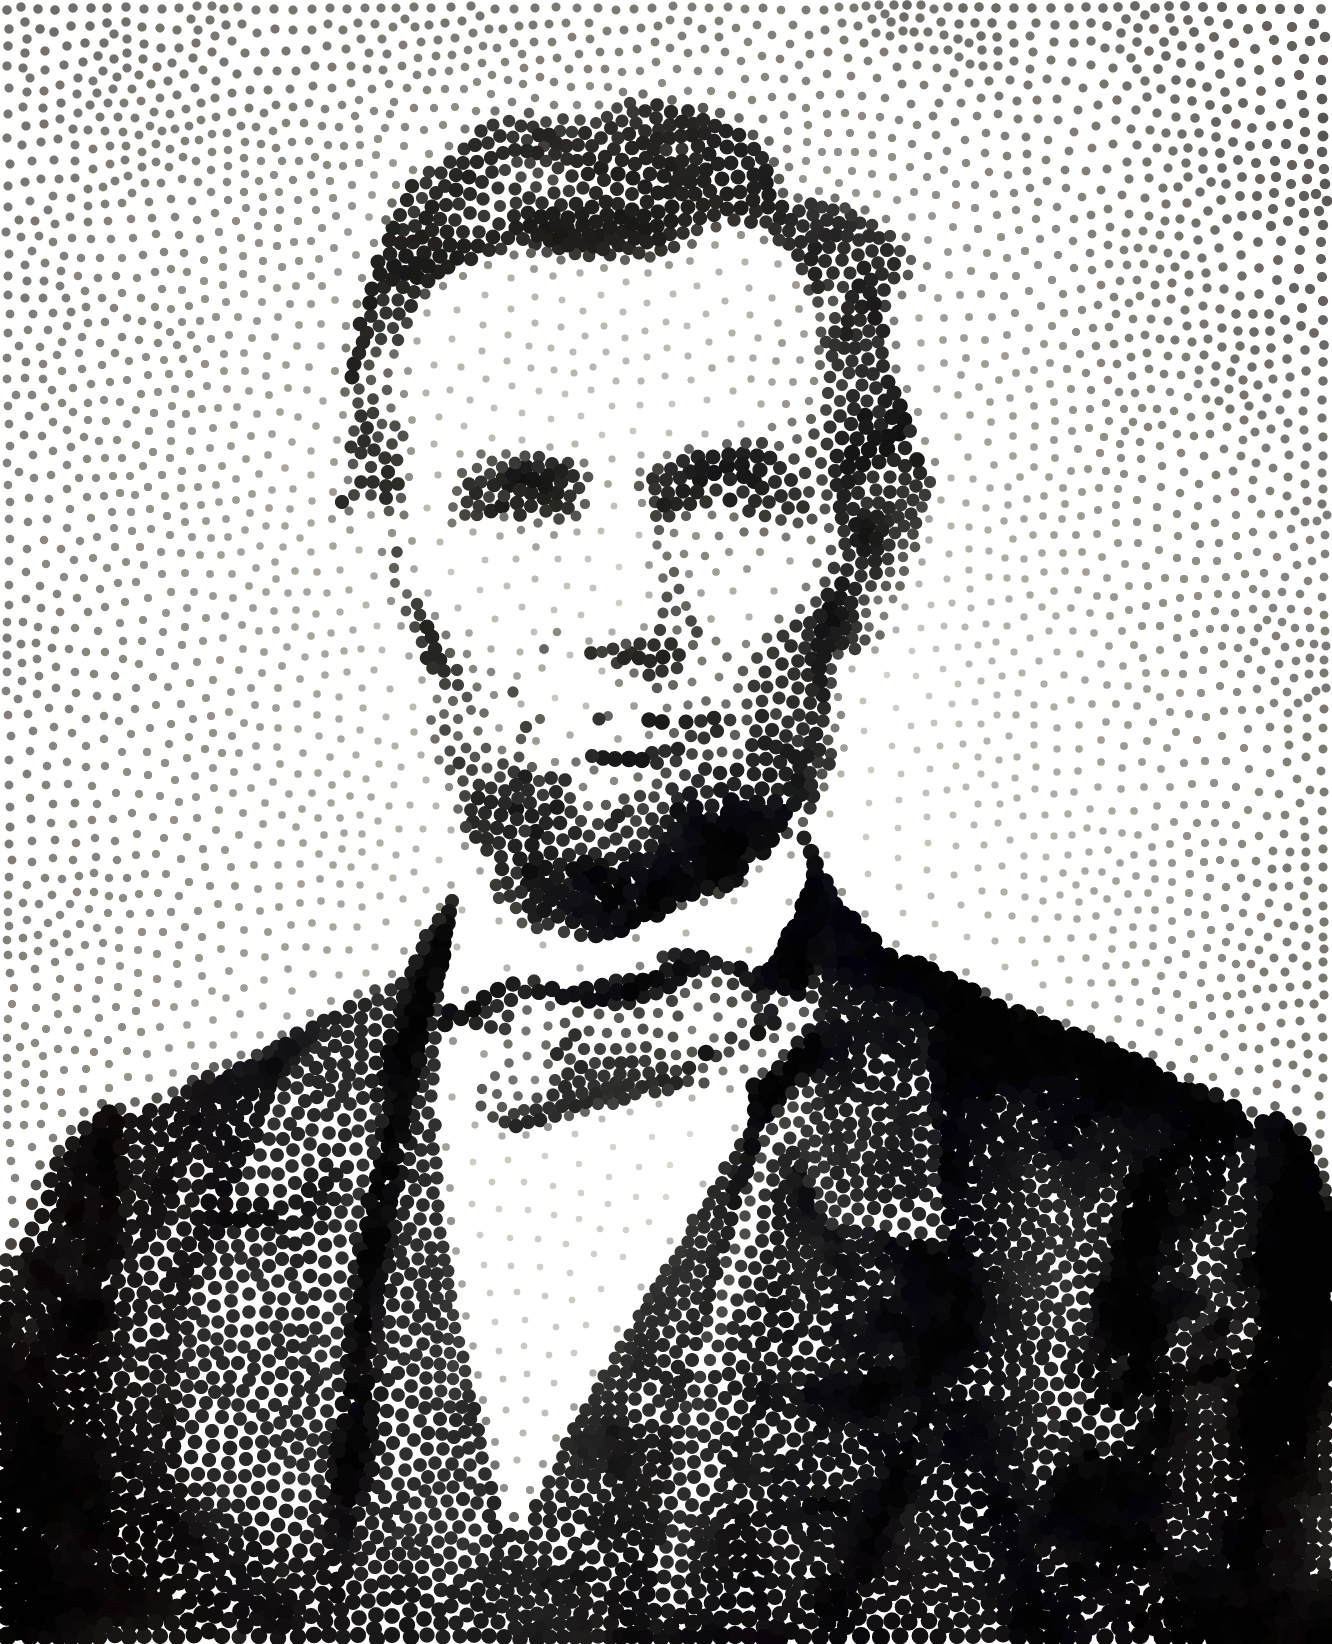
\includegraphics[width=\linewidth]{pix/hc_AL_8000_r10.png}
		\caption{HC, 8000px,$r \le 10$}
	\end{subfigure}
	\begin{subfigure}[b]{0.4\linewidth}
		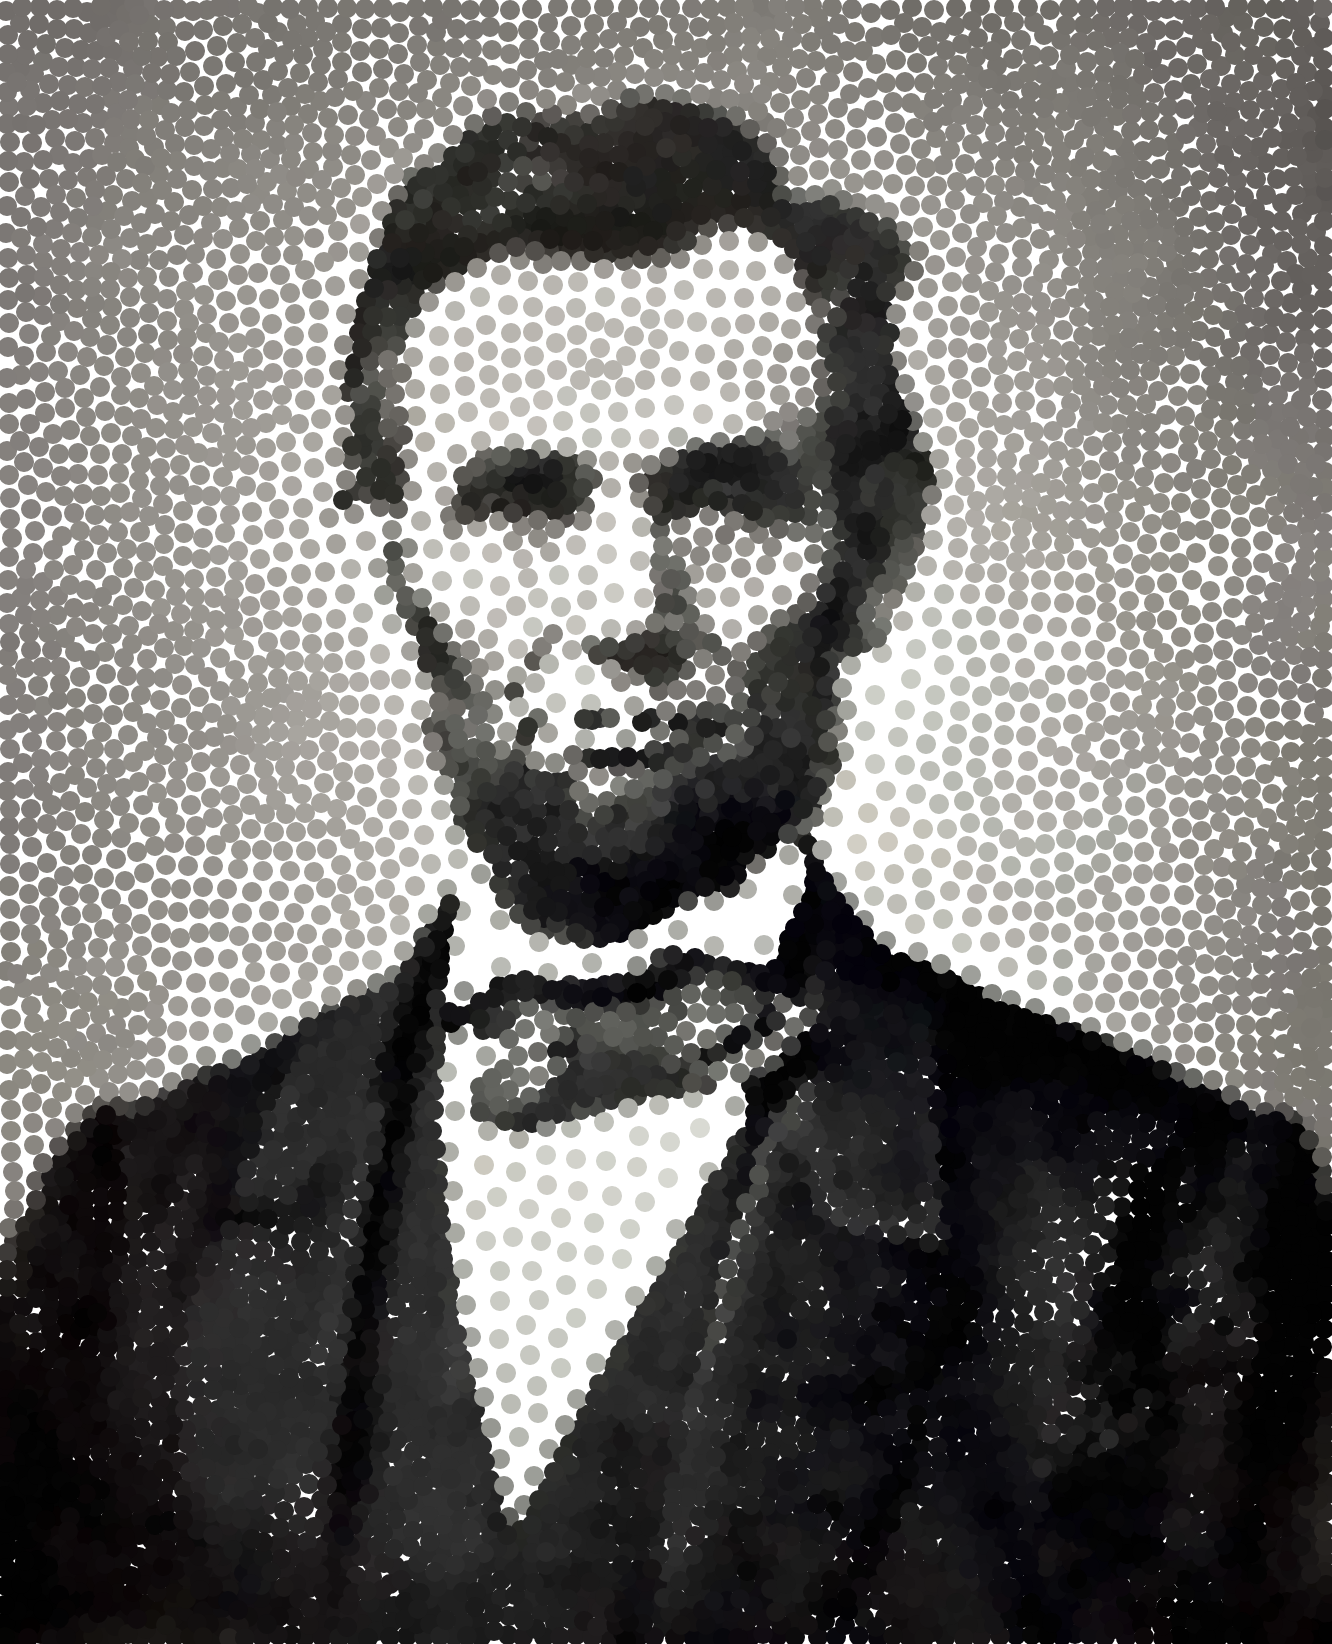
\includegraphics[width=\linewidth]{pix/hc_AL_8000_fixed_10.png}
		\caption{HC, 8000px, r = 10}
	\end{subfigure}
	\begin{subfigure}[b]{0.4\linewidth}
		
\includegraphics[width=\linewidth]{pix/vr_AL_8000_r10.png}
		\caption{VM, 8000px, $r \le 10$}
	\end{subfigure}
	\begin{subfigure}[b]{0.4\linewidth}
		
\includegraphics[width=\linewidth]{pix/vr_AL_8000_fixed_10.png}
		\caption{VM, 8000px, r = 10}
	\end{subfigure}
	\caption{Variations between fixed and uniform disk radius between methods. 8000 disks.}
	\label{fig:vr_hc_fixed}
\end{figure}

The images in Figure \ref{fig:vr_hc_fixed} are variations of an 8000 point stipling of the sampled image. The top row utilizes HC, while the bottom row uses VR. The left two images have variable stipple sizes, while the images on the right have a fixed stipple radius of 10 pixels. Image a) maintains many of thestrong  edge detais of the original at the expense of some of the finer details, such as the lips. Figure c) mainains much of the finere details, but the contrasts between lighter and darker areas lose much of their distinction. Of the four images, d) is the poorest quality as the fixed stipple size causes many of the subptle shades of gray to be completely lost. 

\subsection{Variations on Speed with Number of Disks}
As the two methods used in this assignment differ signicantly, the time to calculate a solution does vary within each implementation. This variation is dependant upon the number of disls selected to stipple the given image. As seen in the following table, run times for HC increase with increased number of disks. The VM, however, has the opposite trend ... becoming faster as disk count increases. This is due to the larger number of individual pixels that must be handled and calculated even at smaller quantities of disks.

\begin{table}
\centering
\caption{Sampling of HC and VR run times versus disk quantities.}
\label{table1}
	\begin{tabular}{ | l | l | p{1.8cm} |}
	\hline
	Disks & hedcuter (s) & voronoi (s) \\ \hline
	1000 & 384.581 & 121.74 \\ \hline
	2000 & 417.722 & 70.80 \\ \hline
	4000 & 411.796 & 50.76 \\ \hline
	8000 & 732.592 & 38.16 \\ \hline
	16000 & 1325.6 & 27.91 \\ \hline
	32000 & 1381.59 & 20.31 \\ \hline
	64000 & 2052.16 & 16.59 \\ \hline
	128000 & 3961.65 & 15.68 \\ \hline
	\end{tabular}
\end{table}

\subsection{Differences in image type}

\subsection{Differences from WSJ Hedcuts}
The images produced by HC and VM differ from the traditional Wall Street Journal hedcuts is a couple of areas. First, and simplest, are background areas. The subject mater for a WSJ hedcut is usually a person, and just the head and upper torso are included. For a grayscale image, the background would be included to some extent - even when unwanted. This can be avoided somewhat by avoiding darker backgrounds.

Another differene is the us of random samples. When an artist creates a hedcut, there is purpose behind the stipples produced. From a programmatic standpoint, there will always be "artifacts" - unwanted pixels in the image as a result of the processing. These, too, may be eliminated though careful image selection and image quality.
Random Samples

\section{Improvement of hedcuter method}

\subsection{Distribution of Disks}
Stictly random selection of initial points. How does this affect the edges?

\subsection{Improve efficiency}
GPU use - i never could get this to work on my Macbook Pro.


\subsection{Colorful Disks}
Addition of "colorful" disks.


\begin{figure}[H]
	\centering
	\begin{subfigure}[b]{0.84\linewidth}
		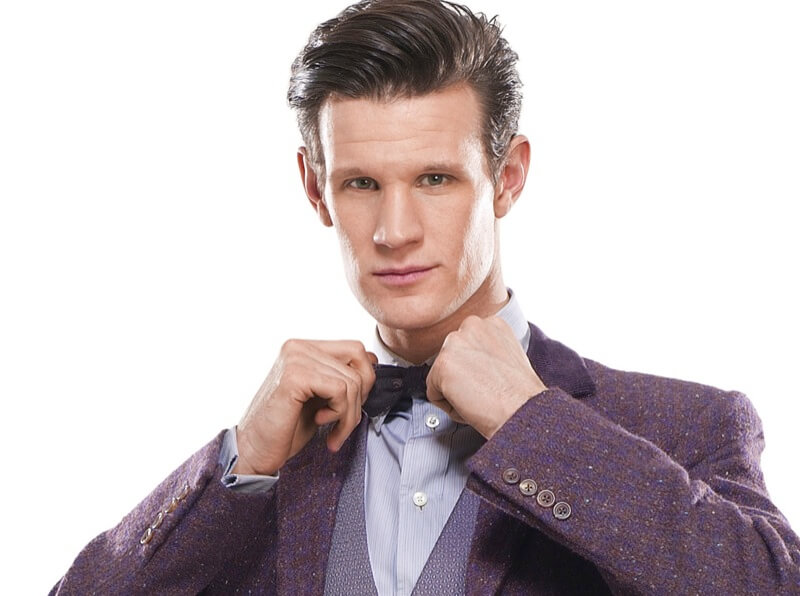
\includegraphics[width=\linewidth]{pix/bowtie.png}
		\caption{Original Image: 800x596, RGB}
	\end{subfigure}
	\begin{subfigure}[b]{0.4\linewidth}
		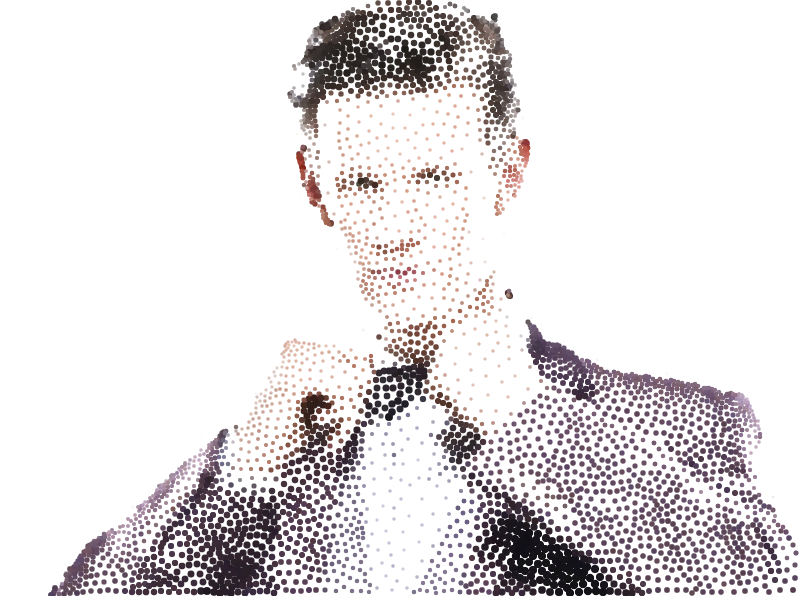
\includegraphics[width=\linewidth]{pix/hc_bowtie-4000.png}
		\caption{HC, 4000px, native colored stipples}
	\end{subfigure}
	\begin{subfigure}[b]{0.4\linewidth}
		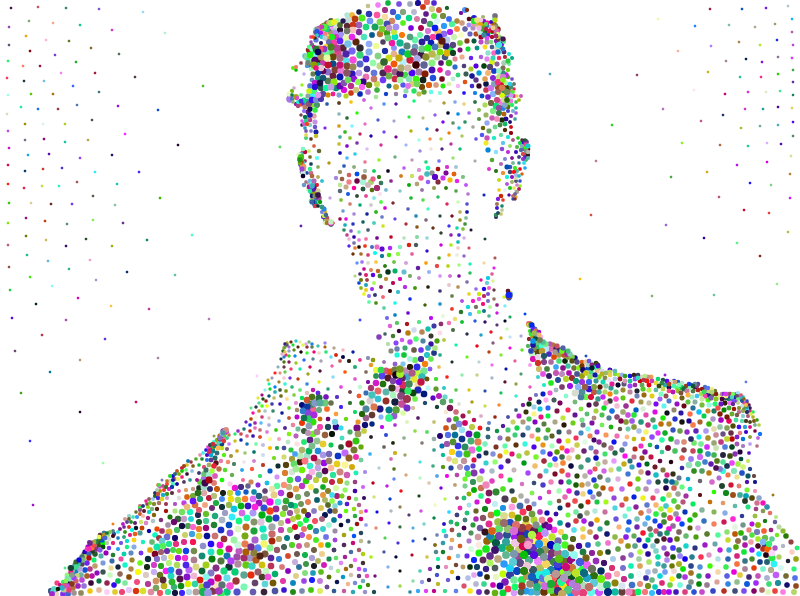
\includegraphics[width=\linewidth]{pix/hc_bowtie-4000_color}
		\caption{VM, 4000px, colorful disks}
	\end{subfigure}
	\caption{Variations of applying random colorization to output disks.}
	\label{fig:bowties}
\end{figure}

As seen in Figure \ref{fig:bowties}, the underlying pixel color is used when the image selected for stippling is itself a color image. Adding a few randomizers behind the selction of the color of each indivifual pixel yield an extremely colorful stippling.

The following shows the Original and the Modified code snippettes which produced the colorful stipplings in Figure \ref{fig:bowties}.

Original:
\begin{lstlisting}
r = floor(r / cell.coverage.size());
g = floor(g / cell.coverage.size());
b = floor(b / cell.coverage.size());
\end{lstlisting}

Moddified:
\begin{lstlisting}
r = (int)floor(255*rng_uniform.uniform(0.f, 1.f));
g = (int)floor(255*rng_uniform.uniform(0.f, 1.f));
b = (int)floor(255*rng_uniform.uniform(0.f, 1.f));
\end{lstlisting}

\bibliographystyle{plain}
\bibliography{report}

\end{document}


